\documentclass{article}
\usepackage{graphicx} % Required for inserting images
\usepackage[utf8]{inputenc}
\usepackage{amsmath}
\usepackage{graphicx}
\usepackage{tikz}
\usepackage{array}
\usetikzlibrary{trees}
\usepackage{amssymb}
\usepackage{amsthm}
\usepackage{multirow}
\usepackage{dcolumn}
\usepackage{verbatim}
\usepackage{booktabs}

\newcolumntype{2}{D{.}{}{2.0}}

\title{CSC279 HW5}
\author{Hanzhang Yin}
\date{Nov/13/2023}

\begin{document}

\maketitle

\subsection*{Collaborator}
Chenxi Xu, Yekai Pan, Yiling Zou, Boyi Zhang

\subsection*{PROBLEM 15---Closest point, farthest point.}
\\
\textbf{Answer: }

\begin{enumerate}
    \item Assume $q$ is inside $P$. We want to find the closest point to $q$ in $\{p_1, \dots, p_n\}$.
    \\
    \textbf{Reasoning: }
    \\
    
    \item Assume $q$ is outside $P$. We want to find the closest point to $q$ in $\{p_1, \dots, p_n\}$.
    \item Assume $q$ is inside $P$. We want to find the farthest point to $q$ in $\{p_1, \dots, p_n\}$.
    \item Assume $q$ is outside $P$. We want to find the farthest point to $q$ in $\{p_1, \dots, p_n\}$.
    \item Assume $q$ is inside $P$. We want to find the closest point to $q$ on $P$.
    \item Assume $q$ is outside $P$. We want to find the closest point to $q$ on $P$.
    \item Assume $q$ is inside $P$. We want to find the farthest point to $q$ on $P$.
    \item Assume $q$ is outside $P$. We want to find the farthest point to $q$ on $P$.
\end{enumerate}

\\
\textbf{Question 1 - 4 Reasoning: }
For Problems 1--4, the distances from \( q \) to the vertices \( p_i \) do not exhibit a unimodal or monotonic pattern along the ordered sequence of vertices because convex polygons can be irregular, causing the distances to fluctuate unpredictably. This lack of a consistent pattern means we cannot apply efficient search algorithms like binary or ternary search, which rely on such properties. Consequently, to find the closest or farthest vertex, we must individually compute and compare the distances for all \( n \) vertices, leading to a time complexity of \( \Omega(n) \) for each problem.
\\
\textbf{Question 5 - 6 Reasoning: }
\\
The distance from $q$ to the boundary of the convex polygon $P$ is a convex function along the perimeter, regardless of whether $q$ is inside or outside $P$.
(i.e. The distance decreases to a minimum point and then increases, forming a single through)

\begin{enumerate}
    \item \textbf{Problem 5:} \( q \) inside \( P \); find the closest point to \( q \) on \( P \).
    \begin{itemize}
        \item \textbf{Solution:} \( O(\log n) \) time.
        \item \textbf{Reasoning:} Perform binary search over edges to find the closest point where the minimum distance occurs.
    \end{itemize}

    \item \textbf{Problem 6:} \( q \) outside \( P \); find the closest point to \( q \) on \( P \).
    \begin{itemize}
        \item \textbf{Solution:} \( O(\log n) \) time.
        \item \textbf{Reasoning:} Same as Problem 5, use binary search to find the closest point on edges.
    \end{itemize}
\end{enumerate}
\\
\textbf{Question 7 - 8 Reasoning: }
\\
The farthest point from $q$ can lie anywhere along the perimeter of the convex polygon $P$, necessitating a check of all edges and vertices.
The distance function for farthest points is not unimodal, preventing the use of efficient binary or ternary search methods.
Hence, without preprocessing, we need $\Omega(n)$ time to do them.

\begin{enumerate}
    \item \textbf{Problem 7:} \( q \) inside \( P \); find the farthest point from \( q \) on \( P \).
    \begin{itemize}
        \item \textbf{Solution:} \( \Omega(n) \) time.
        \item \textbf{Reasoning:} Requires examining all edges using rotating calipers for antipodal points.
    \end{itemize}

    \item \textbf{Problem 8:} \( q \) outside \( P \); find the farthest point from \( q \) on \( P \).
    \begin{itemize}
        \item \textbf{Solution:} \( \Omega(n) \) time.
        \item \textbf{Reasoning:} Similar to Problem 7, needs \( \Omega(n) \) time to check all edges.
    \end{itemize}
\end{enumerate}

\newpage

\subsection*{PROBLEM 16}

\begin{figure*}[h]
    \centering
    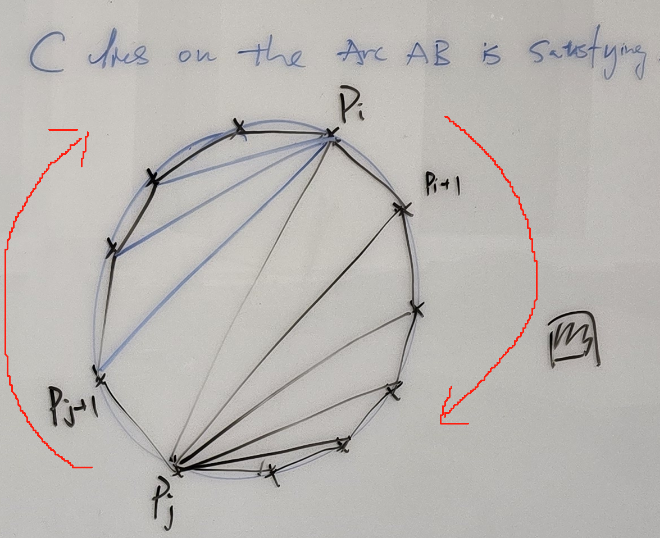
\includegraphics[width=0.7\textwidth]{HW5_Q2.png}
    \label{fig:q2PROOF}
\end{figure*}

\begin{proof}
    Let $\{P_1, \dots, P_n\}$ be the collection of points of a convex polygon $P$.
    \\
    \textbf{Steps for Triangulation: }

    \begin{enumerate}
        \item Order points in clock-wise order $\{p_1, ..., p_n\}$.

        \item Pick the \textbf{longest side} from \textbf{diagonal} or \textbf{side} of $P$: $P_i, P_j$.

        \item Pick the third point $P_k$ such that $P_k$ is the neighbor of point $p_i$ OR $p_j$. WLOG, 
        pick the neighbor of $p_i$ as the third point. We denote the third point as $P_{i+1}$ or $P_{j-1}$.
        \textbf{Note:} This $P_k$ is on the opposite arc from $P_i P_j$.
        \item Form the first triangle as $\triangle P_i P_j P_k$:
        \begin{enumerate}
            \item Then we iteratively add the rest of the polygon of the ``half'' of the polygon as:
            \\
            \textbf{Note:} The neighbor of $P_{i + n}$ is $P_{j - 1}$ and $P_{j - 3}$.
            \[
                P_j P_{j+1} P_{j+2}, \dots, P_{j} P_{i + n} P_{j-1}
            \]

            \item For the rest of the ``half'' of the polygon:
            \\
            \textbf{Note:} The neighbor of $P_{j + m}$ is $P_{i - 1}$ and $P_{i - 3}$.
            \[
                P_i P_j P_{j+1}, \dots, \dots, P_{i} P_{j + m} P_{i-1}.
            \]
        \end{enumerate}
\end{enumerate}

\end{proof}

\subsection*{PROBLEM 17}
First construct the Voronoi diagram. For every edge e, we calculate the minimum distance d between e to the Voronoi sites pi and pk that use e as an edge. If $d > (2c + l) / 2$, then we set $i$ and $k$ as good.
\\
\begin{verbatim}
func (P: set of points,c , l):
    # Avoid replicate side being added
    ans = set()
    # return vornoi diagram of point p
    # O(nlogn)
    v = vornoi_diagram(P)
    # O(n)
    for edge in v.E:
        # traverse all the edge, compute the distance between the corresponding point and the edge
        distance = compute(edge) 
        if distance < (2c + l):
            ans.append(edge.p1)
            ans.append(edge.p2)
    return ans
\end{verbatim}

\begin{verbatim}
Input: 
points: list of n points p1, p2, ..., pn in the plane
r: radius of each circle Ci centered at pi
l: radius of the circle to be found

Output: 
    GoodIndices: list of indices i where pi is good

Algorithm FindGoodPoints(points, r, l):
    1. Compute the Voronoi diagram VD of the points p1, ..., pn.
    # This can be done in O(n log n) time.

    2. Initialize GoodIndices as an empty list.

    
    3. For each point pi in points:
    # This can be done in O(n) time.
        a. Let V_i be the Voronoi cell of pi in Voronoi Diagram.
        b. Let C_i be the circle centered at pi with radius l + r.
        c. Initialize IsGood[i] = False.

        d. For each edge e of V_i:
            i.   If e is a finite line segment between vertices v1 and v2:
                 - Compute the intersection points between e and C_i.
                 - If there is an intersection:
                     - Set IsGood[i] = True.
                     - Break out of the edge loop.
            ii.  If e is an infinite ray (unbounded edge):
                 - Compute the intersection between e and C_i if it exists.
                 - Same as above.

        e. If IsGood[i] is False:
            - For each vertex v in V_i:
                - If v lies inside C_i:
                    - Set IsGood[i] = True.
                    - Break out of the vertex loop.

        f. If IsGood[i] is True:
            - Append i to GoodIndices.

    4. Return GoodIndices.
\end{verbatim}

\subsection*{PROBLEM 18}

\textbf{Result: }
\\
\begin{table}[h!]
    \centering
    \begin{tabular}{@{}cccc@{}}
    \toprule
    \textbf{Processing \( n \)} & \textbf{Max Depth} & \textbf{Avg Depth} \\ \midrule
    10 & 8  & 5.45273631840796 \\
    20 & 12 & 7.750312109862672 \\
    30 & 18 & 8.939478067740144 \\
    40 & 17 & 9.610121836925961 \\
    50 & 21 & 9.93361327734453 \\ \bottomrule
    \end{tabular}
    \caption{Depth statistics for different values of \( n \)}
\end{table}

\begin{figure*}[h]
    \centering
    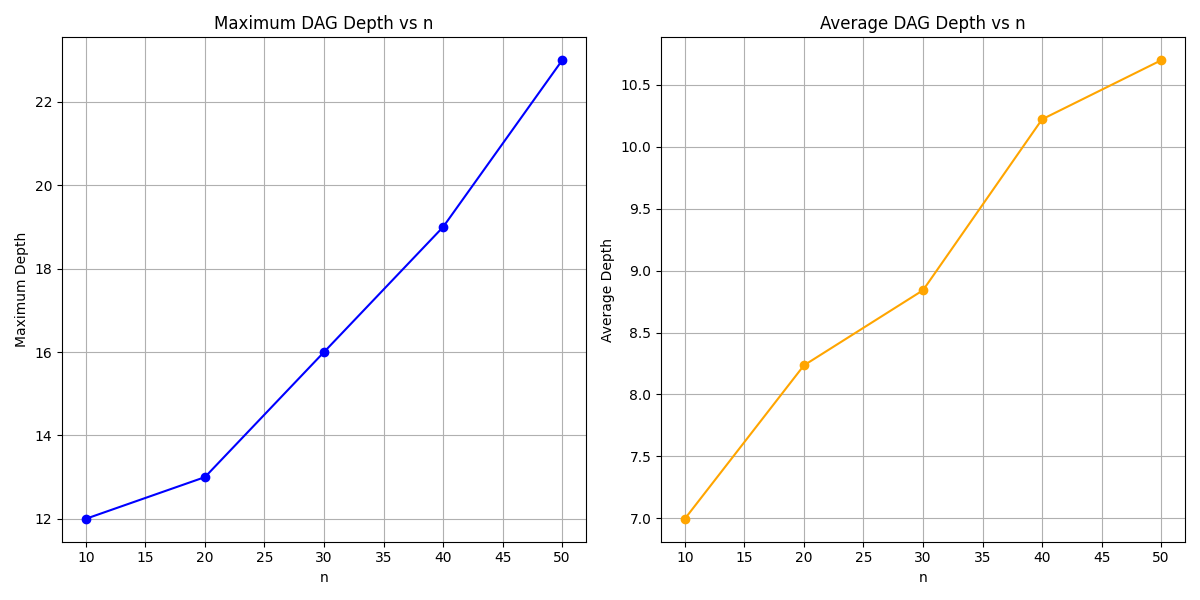
\includegraphics[width=0.9\textwidth]{Figure_1.png}
    \label{fig:model}
\end{figure*}

\hspace{0.01cm}
\\
\textbf{Short Analysis: }
\\
The result I got is reasonable, with the average depths increasing in $log n$ as expected, indicating that the algorithm effectively maintains a balanced DAG structure. 
Although the maximum depths are somewhat higher than theoretical predictions, they remain within an acceptable range considering the algorithm's randomness and the potential for local depth increases during edge legalization. 
\\
\textbf{Implementation: }
\\
The following code of randomized Delaunay triangulation algorithm with history DAG was implemented in Python:
\begin{verbatim}
# Data Structures Definitions

class Point:
    def __init__(self, x, y):
        self.x = x
        self.y = y

class SegmentWrapper:
    """
    Helper class to uniquely identify a segment irrespective of point order.
    """
    def __init__(self, p1, p2):
        # Ensure consistent ordering
        if (p1.x, p1.y) < (p2.x, p2.y):
            self.p1, self.p2 = p1, p2
        else:
            self.p1, self.p2 = p2, p1

    def __eq__(self, other):
        return (self.p1.x, self.p1.y) == (other.p1.x, other.p1.y) and \
               (self.p2.x, self.p2.y) == (other.p2.x, other.p2.y)

    def __hash__(self):
        return hash(((self.p1.x, self.p1.y), (self.p2.x, self.p2.y)))

    def __repr__(self):
        return f"Segment(({self.p1.x}, {self.p1.y}) - ({self.p2.x}, {self.p2.y}))"

class Triangle:
    def __init__(self, p1, p2, p3):
        self.vertices = [p1, p2, p3]  # Points
        self.edges = [
            SegmentWrapper(p1, p2),
            SegmentWrapper(p2, p3),
            SegmentWrapper(p3, p1)
        ]
        self.neighbors = {}  # edge -> adjacent triangle
        self.children = []  # For history DAG

    def contains_point(self, point):
        return point in self.vertices

    def __repr__(self):
        verts = ', '.join([f"({p.x}, {p.y})" for p in self.vertices])
        return f"Triangle({verts})"

class HistoryDAGNode:
    def __init__(self, triangle):
        self.triangle = triangle  # Triangle object
        self.children = []        # List of HistoryDAGNode

    def add_child(self, child_node):
        self.children.append(child_node)

# Delaunay Triangulation Class

class DelaunayTriangulation:
    def __init__(self, points):
        self.points = points  # List of Point objects
        self.segments = {}    # SegmentWrapper -> list of adjacent Triangles
        self.triangles = []   # List of Triangle objects
        self.history_root = None

    def create_super_triangle(self):
        """
        Create a super-triangle that encompasses all the points.
        """
        min_x = min(p.x for p in self.points)
        max_x = max(p.x for p in self.points)
        min_y = min(p.y for p in self.points)
        max_y = max(p.y for p in self.points)

        dx = max_x - min_x
        dy = max_y - min_y
        delta_max = max(dx, dy) * 100  # Make it large enough

        # Create three points that form a super-triangle
        p1 = Point(min_x - delta_max, min_y - delta_max)
        p2 = Point(min_x + 2 * delta_max, min_y - delta_max)
        p3 = Point(min_x - delta_max, max_y + 2 * delta_max)

        super_triangle = Triangle(p1, p2, p3)
        self.triangles.append(super_triangle)
        self.history_root = HistoryDAGNode(super_triangle)

        # Add segments of the super-triangle
        for edge in super_triangle.edges:
            self.segments.setdefault(edge, []).append(super_triangle)

    def locate_containing_triangle(self, point):
        """
        Traverse the history DAG to locate the triangle containing the point.
        """
        node = self.history_root
        while node.children:
            found = False
            for child in node.children:
                if self.point_in_triangle(point, child.triangle):
                    node = child
                    found = True
                    break
            if not found:
                break  # Point not found in any child; fallback
        # Now, node.triangle should contain the point
        return node.triangle, node

    @staticmethod
    def point_in_triangle(p, triangle):
        """
        Check if point p is inside the given triangle using barycentric coordinates.
        """
        def sign(p1, p2, p3):
            return (p1.x - p3.x) * (p2.y - p3.y) - \
                   (p2.x - p3.x) * (p1.y - p3.y)

        b1 = sign(p, triangle.vertices[0], triangle.vertices[1]) < 0.0
        b2 = sign(p, triangle.vertices[1], triangle.vertices[2]) < 0.0
        b3 = sign(p, triangle.vertices[2], triangle.vertices[0]) < 0.0

        return ((b1 == b2) and (b2 == b3))

    def insert_point(self, point):
        """
        Insert a single point into the triangulation.
        """
        containing_triangle, containing_node = self.locate_containing_triangle(point)

        # Remove the containing triangle
        self.triangles.remove(containing_triangle)

        # Create new triangles by connecting the point 
        # to the vertices of the containing triangle
        t1 = Triangle(point, containing_triangle.vertices[0], 
            containing_triangle.vertices[1])
        t2 = Triangle(point, containing_triangle.vertices[1], 
            containing_triangle.vertices[2])
        t3 = Triangle(point, containing_triangle.vertices[2], 
            containing_triangle.vertices[0])

        # Set neighbors
        self.set_neighbors(t1, containing_triangle)
        self.set_neighbors(t2, containing_triangle)
        self.set_neighbors(t3, containing_triangle)

        # Add new triangles
        self.triangles.extend([t1, t2, t3])

        # Update segments
        for t in [t1, t2, t3]:
            for edge in t.edges:
                self.segments.setdefault(edge, []).append(t)

        # Update history DAG
        child_nodes = [
            HistoryDAGNode(t1),
            HistoryDAGNode(t2),
            HistoryDAGNode(t3)
        ]
        for child in child_nodes:
            containing_node.add_child(child)

        # Edge Legalization
        for t in [t1, t2, t3]:
            for edge in t.edges:
                if point in [edge.p1, edge.p2]:
                    self.legalize_edge(edge, t, point)

    def set_neighbors(self, new_triangle, old_triangle):
        """
        Set the neighboring triangles for the new triangle.
        """
        for edge in new_triangle.edges:
            if edge in self.segments:
                for neighbor in self.segments[edge]:
                    if neighbor != old_triangle and neighbor != new_triangle:
                        new_triangle.neighbors[edge] = neighbor
                        neighbor.neighbors[edge] = new_triangle

    def legalize_edge(self, edge, triangle, point):
        """
        Legalize an edge to restore the Delaunay condition.
        """
        if edge not in triangle.neighbors:
            return  # Boundary edge

        neighbor = triangle.neighbors[edge]
        if neighbor is None:
            return

        # Find the opposite point in the neighbor triangle
        opposite_point = [v for v in neighbor.vertices 
                            if v not in [edge.p1, edge.p2]][0]

        if self.in_circumcircle(opposite_point, triangle):
            # Perform edge flip
            new_triangles = self.edge_flip(triangle, neighbor, edge, 
                                            point, opposite_point)
            for new_t in new_triangles:
                for e in new_t.edges:
                    if point in [e.p1, e.p2]:
                        self.legalize_edge(e, new_t, point)

    def edge_flip(self, t1, t2, edge, point, opposite_point):
        """
        Flip the shared edge between two triangles.
        """
        # Remove old triangles
        self.triangles.remove(t1)
        self.triangles.remove(t2)

        # Remove edge from segments
        self.segments[edge].remove(t1)
        self.segments[edge].remove(t2)
        if not self.segments[edge]:
            del self.segments[edge]

        # Create new edge
        new_edge = SegmentWrapper(point, opposite_point)

        # Create new triangles
        new_t1 = Triangle(point, edge.p1, opposite_point)
        new_t2 = Triangle(point, opposite_point, edge.p2)

        # Update segments
        for t in [new_t1, new_t2]:
            for e in t.edges:
                self.segments.setdefault(e, []).append(t)

        # Update neighbors
        self.update_neighbors_after_flip(t1, t2, new_t1, new_t2, edge, new_edge)

        # Add new triangles
        self.triangles.extend([new_t1, new_t2])

        # Update history DAG
        parent_node = HistoryDAGNode(None)
        t1_node = self.find_history_node(self.history_root, t1)
        t2_node = self.find_history_node(self.history_root, t2)
        parent_node.add_child(t1_node)
        parent_node.add_child(t2_node)
        new_t1_node = HistoryDAGNode(new_t1)
        new_t2_node = HistoryDAGNode(new_t2)
        parent_node.add_child(new_t1_node)
        parent_node.add_child(new_t2_node)

        return [new_t1, new_t2]

    def update_neighbors_after_flip(self, t1, t2, new_t1, new_t2, old_edge, new_edge):
        """
        Update neighbor relationships after an edge flip.
        """
        # Set neighbors for new_t1
        new_t1.neighbors[new_edge] = new_t2
        new_t2.neighbors[new_edge] = new_t1

        # Update other neighbors
        for e in new_t1.edges:
            if e != new_edge:
                for neighbor in self.segments[e]:
                    if neighbor != new_t1:
                        new_t1.neighbors[e] = neighbor
                        neighbor.neighbors[e] = new_t1

        for e in new_t2.edges:
            if e != new_edge:
                for neighbor in self.segments[e]:
                    if neighbor != new_t2:
                        new_t2.neighbors[e] = neighbor
                        neighbor.neighbors[e] = new_t2

    def find_history_node(self, node, triangle):
        """
        Find the history DAG node corresponding to the given triangle.
        """
        if node.triangle == triangle:
            return node
        for child in node.children:
            result = self.find_history_node(child, triangle)
            if result is not None:
                return result
        return None

    def in_circumcircle(self, point, triangle):
        """
        Check if a point is inside the circumcircle of a triangle.
        """
        ax, ay = triangle.vertices[0].x - point.x, triangle.vertices[0].y - point.y
        bx, by = triangle.vertices[1].x - point.x, triangle.vertices[1].y - point.y
        cx, cy = triangle.vertices[2].x - point.x, triangle.vertices[2].y - point.y

        det = (ax * (by * (cx**2 + cy**2) - cy * (bx**2 + by**2)) -
               ay * (bx * (cx**2 + cy**2) - cx * (bx**2 + by**2)) +
               (ax**2 + ay**2) * (bx * cy - cx * by))

        return det > 0

    def build_triangulation(self):
        """
        Build the triangulation by inserting all points.
        """
        self.create_super_triangle()
        for point in self.points:
            self.insert_point(point)
        self.remove_super_triangle()

    def remove_super_triangle(self):
        """
        Remove any triangles that share a vertex with the super-triangle.
        """
        # Super-triangle vertices
        super_vertices = set(self.history_root.triangle.vertices)
        self.triangles = [t for t in self.triangles 
                            if not any(v in super_vertices for v in t.vertices)]

    def calculate_dag_depths(self):
        """
        Calculate maximum and average depths of the history DAG.
        """
        depths = []
        queue = deque([(self.history_root, 0)])

        while queue:
            node, depth = queue.popleft()
            if not node.children:
                depths.append(depth)
            else:
                for child in node.children:
                    queue.append((child, depth + 1))

        max_depth = max(depths) if depths else 0
        avg_depth = sum(depths) / len(depths) if depths else 0
        return max_depth, avg_depth
    
    def plot_triangulation(self):
        """
        Plot the triangulation.
        """
        plt.figure(figsize=(8, 8))
        for triangle in self.triangles:
            x_coords = [vertex.x for vertex in triangle.vertices + [triangle.vertices[0]]]
            y_coords = [vertex.y for vertex in triangle.vertices + [triangle.vertices[0]]]
            plt.plot(x_coords, y_coords, 'k-')
        plt.scatter([p.x for p in self.points], 
                    [p.y for p in self.points], color='red', s=10)
        plt.axis('equal')
        plt.title('Delaunay Triangulation')
        plt.show()
\end{verbatim}


\end{document}
